\section{Texto Texto Texto}
\label{motivacao}

Texto texto texto texto texto texto texto texto texto texto texto texto texto texto texto texto texto texto texto texto texto texto texto texto texto texto texto texto texto texto texto texto texto texto texto texto, \textbf{exemplo} sigla \gls{UFPE}.

%você pode organizar melhor suas imagens se criar subpastas nos chapters
\begin{figure}[ht!]
\centering

\caption{\textmd{Texto Texto Texto Texto Texto Texto Texto Texto Texto Texto Texto Texto Texto Texto Texto Texto Texto Texto Texto Texto Texto Texto Texto Texto Texto Texto Texto Texto}}
\label{fig:figuraex}
\fcolorbox{gray}{white}{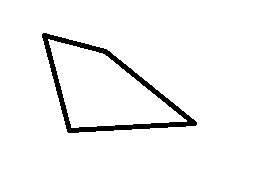
\includegraphics[width=0.5\textwidth]{images/captitulo1/figuraex.png}}

\fonteref{\citeauthor{manualufpe2020} (\citeyear{manualufpe2020})}
\end{figure}

Texto texto texto texto texto texto texto texto texto texto texto texto texto texto texto texto texto texto texto texto texto texto texto texto texto texto texto texto texto texto texto texto texto texto texto texto, conforme Figuras \ref{fig:figuraex} e Figuras \ref{fig:figuraex2} e também Grafico \ref{graph:grafico1}, continua no Capítulo \ref{chap:outrocapitulo}.


\begin{figure}[ht!]
\centering

\caption{\textmd{Texto Texto Texto Texto Texto Texto Texto}}
\label{fig:figuraex2}
\fcolorbox{gray}{white}{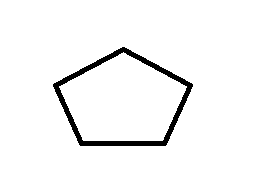
\includegraphics[width=0.80\textwidth]{images/captitulo1/figuraex2.png}}

\fonteadapt{\citeauthor{manualufpe2020} (\citeyear{manualufpe2020})}
\end{figure}

Texto texto texto texto texto texto texto texto texto texto texto texto texto texto texto texto texto texto texto texto texto texto texto texto texto texto texto texto texto texto texto texto texto texto texto texto texto texto texto texto texto texto texto texto texto texto texto texto texto texto texto texto texto texto texto texto texto texto texto texto texto texto texto texto texto texto texto texto texto texto texto texto texto texto texto texto texto texto texto texto texto \gls{UFPE}.

\begin{grafico}[ht!]
\centering

\caption{\textmd{Texto Texto Texto Texto Texto Texto Texto}}
\label{graph:grafico1}
\fcolorbox{gray}{white}{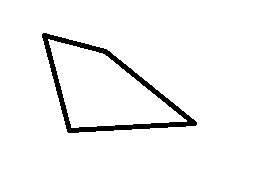
\includegraphics[width=0.80\textwidth]{images/captitulo1/figuraex.png}}

\par\medskip\ABNTEXfontereduzida\selectfont\textbf{Fonte:} \citeauthor{manualufpe2020} (\citeyear{manualufpe2020}) \par\medskip
\end{grafico}

Texto texto texto texto texto texto texto texto texto texto texto texto texto texto texto texto texto texto texto texto texto texto texto texto texto texto texto \gls{UFPE}.
